% $Id$

\section{Construction of Inspiral Pipelines}
\label{s:construction}

Chapter \ref{ch:findchirp} described the algorithms that we use to generate
inspiral triggers for an inspiral template from a single data segment.
However, there is more to searching for binary coalescences than inspiral
trigger generation. To perform a search for a given class of sources in a
large quantity of interferometer data we construct a \emph{detection
pipeline}. In this chapter we describe the pipeline that has been constructed
to search for binary neutron stars and binary black hole MACHOs in the S2
data.

A detection pipeline is a sequence of operations that starts with the raw data
from the interferometers and produces a list of \emph{candidate events}.
Figure \ref{f:simple_pipe} shows a simple pipeline to filter the data from a
pair of interferometers labelled $1$ and $2$. In this section, we will give an
overview of the pipeline and the following sections describe each component in
more detail. 

We first consider the data from the interferometers. In order to analyze
data, it must come from interferometers in stable operation. Running an
interferometer is a complex process that requires \emph{interferometer
operators} trained to align and lock the inteferometers and to monitor the
quality of the data being taken. From a quisecent state, the operators
manually align the optics of the interferometer to within appropriate
parameters. The operators then direct the automated length sensing and control
system to bring the Fabry--Perot cavities into resonance; the beam splitter
is positioned so that the light at the anti-symmetric port is a minimum. The
recycling cavity is then brought into resonance and the interferometer reports
to the operators that it is \emph{locked}.  In conjection with the operators
\emph{scientfic monitors} physically present at the observatory then decide if
the quality of the data being recorded is suitable to be flagged as
\emph{science mode data} and used for gravitational wave analysis.

It is possible that the operators or science monitors may make mistakes in
deciding that data should be flagged as science mode, such as forgetting to
enable calibration lines. There may also be noise sources or transient events
in the data which make it unsuitable for analysis but which are not detectable
in the control room while the data is being taken. To prevent such data from
being using in an astrophysical analysis, we may apply several \emph{data
quality cuts} to discard poor quality data. We may consider the manual
selection of science mode data is the first line of data quality cuts and we
describe other automated tests in section \ref{s:dq} below.

As mentioned above, the matched filtering described in the previous chapter
generates triggers for a single inspiral template. We generally wish to search
the data for a class of signals. In this thesis, we describe searching for
gravitational waves from binary neutron stars and binary black hole MACHOs.
Both sources use the second order post-Newtonian stationary phase templates
described in chapter \ref{ch:inspiral} and the search algorithms described in
chapter \ref{ch:findchirp}. However, possible template paramters cover
distinct regions of the template parameter space, described by the component
masses $m_1$ and $m_2$. This means that we are searching for signals from a 
region of parameter space, rather than a single template. To do this we
construct a \emph{bank} of inspiral templates as described in section
\ref{s:pipetemplate}. The template bank covers the parameter space of interest, so
that we do not discard any signals from our desired population.

We then use the template bank to filter the data for inspiral signals using
the matched filter and $\chi^2$ veto. This generates a list of \emph{inspiral
triggers} for each interferometer. In figure \ref{f:simple_pipe} a template
bank is generated for each interferometer and the data from an interferometer
filterer through the bank particular to that data. This is not the only method
of generating inspiral triggers in a pipeline, as we will see later. Section
\ref{s:templated} described in more detail how the trigger generation is used
in a pipeline.

One of the most poweful methods of rejecting false alarms is coincidence
between different interferometers. As described previously, there are three
LIGO interferometers which are operated simultaneously during science runs.
The interferometers are named H1, H2 and L1. The H1 and H2 detectors are
$4$~km and $2$~km long interferometers, respectively, co-located to the LIGO
Hanford Observatory. The L1 detector is a $4$~km long interferometer located
at the LIGO Livingston Observatory. A true gravitational wave should be found
in all operating detectors at the same time, up to the error in measurement of
arrival time and the time it takes a gravitational wave to propagate between
the observatories. The time difference between gravitational wave arrival time
may be between $0$~seconds, if the gravitational wave is propagating
perpendicular to a line joining the detectors, or $10$~ms if the gravitational
wave is propagating parrallel to a line joining the detectors. The maximum
time difference comes from the time it takes a gravitational wave to propagate
between the observatories, given by $t = \frac{d}{c}$, where $d = x$~km is the
distance between the observatories and $c$ is the speed of light.This
\emph{time coincidence} test can be applied to inspiral triggers from each
interferometer and is an excellent method of distinguishing real signals from
noise. Other coincidence tests may be used, such as demanding consistency of
the waveform parameters between triggers from two detectors, or consistency in
the recovered amplitude of the signal relative to the sensitivity of the
detectors. We describe these tests and related subtelties in section
\ref{s:coincidence}.

While the goal of the interferometer commissioners and operators is to ensure
that the data recoreded is as stationary and Gaussian as possible, transient
noise sources may still be present in the data. For example it has been seen
that a person jumping up and down in the control room at the observatory will
cause a burst of noise in the gravitational wave channel. There may also be
occasional glitches in the interferometer control systems that cause a
transient in the gravitational wave channel, despite the best efforts of the
experimental team. To allow us to distingish such events from true
gravitational wave signals, we record several thousand data streams of
auxiliary interferometer control channels and physical environmen (PEM)
channels. Auxiliary channels monitor the state of the servo loops that control
the interferometer and include information about the pre-stabilized laser, the
length sensing and control system and the input and output optics. PEM
channels are the data from devices such as siesmometers, magnetometers and
microphones placed in and around the interferometer to detect environmental
sources that may couple to signals in the gravitational wave channel. As
described in section \ref{s:vetoes} this data can be used to construct
\emph{vetoes} on the inspiral triggers. If a coupling can be identified
between a noise source present in an auxiliary or PEM channel and inspiral
triggers in the gravitational wave channel, we may exclude any triggers that
ocour withing some time window of the event in the auxiliary or PEM channel.

The final step in contructing a pipeline is to turn the chosen pipeline
algorithm, such as the one shown in figure \ref{f:simple_pipe}, into code that
can be executed in an automated way on a computing cluster. The execution of
the code must ensures that all the input data has been analyzed in a manner
consistent with the pipeline algorithm. To do this we construct a directed
acyclic graph (DAG) that described the work flow for a specific search on a
data set. For example, we may construct write a DAG to execute the simple
pipeline in figure \ref{f:simple_pipe} on all the data from L1 and H1 recorded
in S2. The DAG decribing the workflow is submitted to a computing cluster and
the Condor high throughput computing system executes that workflow using the
Condor DAG manager. This process is decribed in more detail in section
\ref{s:dag}.

Implict in the above discussion is that fact that there are many parameters
that must be set at each stage of the pipeline. For example: What data quality
cuts should we use? What signal-to-noise and $\chi^2$ thresholds should we use
when generating the inspiral triggers? What coincidence tests should we apply
and what should thier parameters be? What auxiliary channels and PEM channels
should be used and vetoes and how do we apply the vetoes that we choose to
inspiral triggers? Answering these questions is the key to turning a pipeline
into a full binary inspiral search; we call the process of selecting the
paremeters \emph{tuning the pipeline}. In fact, pipeline tuning and
construction of the pipeline are not entirely separate. After constructing a
pipeline and initial tuning, we may decide to revisit the pipeline algorithm
before performing additional tuning.

When tuning the pipeline we may wish to minimize the false alarm rate, that is
minimize the number of candidate events that are not due to inspiral signals.
We may also wish to minimize the false dismissal rate, so ensure that the
pipeline does not discard triggers that are due to real events. We must also
do this in a such a way so that we do not bias our upper limit result. To do
this, we select $10\%$ of all the data that we record as \emph{playground
data}. The data from GPS time $[t,t+1)$ is playground if 
\begin{equation}
t - 700000000  < 600 \quad \mathrm{mod}(6370).
\end{equation}
Playground data is selected algorithmically so as to provide a representative
sample of the full data set. We are free to persue whatever investigations
that we wish on the playground data. We do not use this data in the upper
limit calculation, however we do not preclude the detection of a gravitational
wave signal in this data. We describe the process of tuning the S2 binary
neutron star search in chapter \ref{ch:bns} and the S2 binary black hole MACHO
search in chapter \ref{ch:result}. False alarm rate can be studied by looking
at candidate events in the playground and false dismissal rate can be studied
by \emph{injecting} signals into the data, that is generating a known inspiral
signal and addiing it to the data before passing it through the pipeline.
Injection is decribed in section \ref{s:injections} and chapter
\ref{ch:hardware}.

If we are using data from multiple interferometers, we may measure the
\emph{background rate} of inspiral signals in the data by introducing a time
shift into the data from different detetctors before passing it through the
pipeline. If we assume that noise between the detectors is uncorrelated and
the time shift is sufficiently large, as described in section
\ref{s:background}, then any candidate events that survive the pipeline should
be due to noise alone and not astrophysical signals. By measuring the
background rate, we can measure the false alarm rate of the pipeline which can
be used for both tuning and the computation of the upper limit or detection
confidence.

\begin{figure}[htb]
\label{f:simple_pipe}
\begin{center}
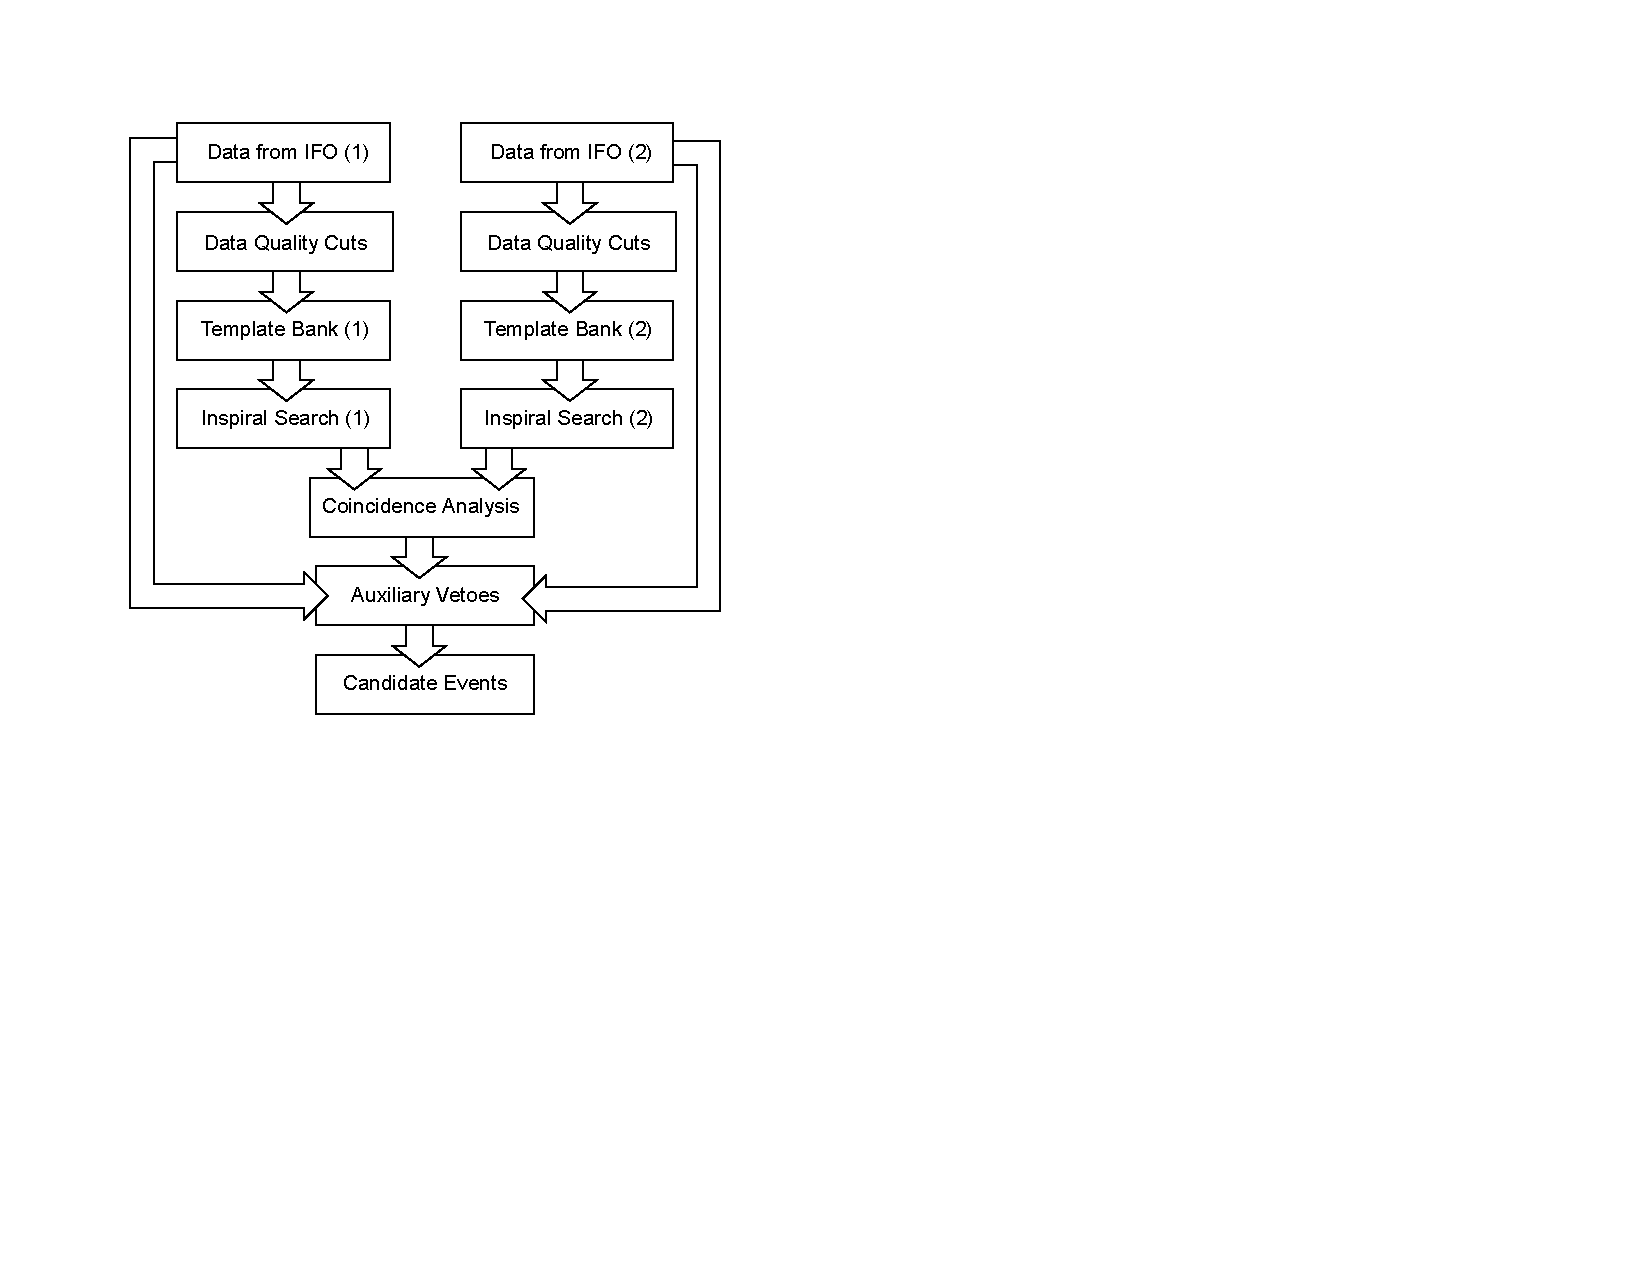
\includegraphics[width=\linewidth]{figures/pipeline/simple_pipe}
\end{center}
\caption{%
An simple pipeline used to search data from two interferometers for inspiral
signals. Raw data from interferometer, labeled $1$ and $2$, is recorded at the
observatories. Data quality cuts are then applied to the raw data to discard
times when the interferometer was not in a stable operating mode. Power
spectra generated from the data are used to generate a template bank for the
inspiral population being searched for. The template banks and interferometer
data are used to generate inspiral triggers for each interferometer. The
triggers for each interferometer are tested for coincidence, as a true
inspiral signal should be present in both interferometers at the same time, up
to the time it takes a gravitational wave to travel between the observatories.
Other coincidence tests, such as waveform parameter consistency, can be
applied at this stage. Transient noise sources may be detected in auxiliary
interferometer channels, for example siesmometers. Such channels may be used to 
veto triggers that survive the coincidence alanysis but are coincidenct with
the signature of noise in the auxiliary channel. Finally we obtain a sample of
candidate events for futher investigation. Each step of the pipeline has many
parameters that can be tuned to minimize the false alarm and false dismissal 
rates.  
}
\end{figure}

\section{Data Quality Cuts}
\label{s:dq}

The inspiral search algorithm is optimized for data with a known,
calibrated noise spectrum which are stationary over the time scale of
the data chunks analyzed ($2048$~s, described in
Section~\ref{ss:analysispipeline}), requiring stable,
well-characterized interferometer performance.  In practice, the
performance is influenced by optical alignment, servo control
settings, and environmental conditions.  We used two strategies to
avoid problematic data.  One was to evaluate {\it data quality} over
relatively long time intervals, using several different tests; time
intervals identified as being suspect or demonstrably bad were skipped
when filtering the data.

Further studies of the raw data yield a series of data quality cuts
that are used to exclude anomalous data from the inspiral
analysis\cite{gwdawveto}. We have excluded times when \emph{(i)} servo
controls in the L1 interferometer were set incorrectly, \emph{(ii)}
calibration information is unavailable for the analysis, \emph{(iii)} there
are photodiode saturations, \emph{(iv)} data has invalid time stamp
information and \emph{(v)} the noise in the H1 interferometer is significantly
larger than average. In general, the interferometer is considered to be
malfunctioning during these times with the exception of \emph{(i)} and
\emph{(ii)} which are due to operator error. In the case of \emph{(v)}, we
ensure that the increased noise is not due to the presence of an inspiral
signal in the data by only excluding times when the noise is excessive for
more than $180$~sec, which is significantly longer that our longest inspiral
signal of $3.7$~sec.

\section{Templated Inspiral Search}
\label{s:pipetemplate}

The previous chaper describe the algorithm that we use to determine if an
inspiral from a binary of masses ${m_1,m_2}$ is present in the interferometer
data. To sumarize, for a given template we use matched filtering to construct
the signal-to-noise ratio, $\rho$, and search for times when this exceeds a
threshold, $\rho > \rho^\ast$. If this happens, we construct a template based
veto, the $\chi^2$ veto\cite{brucechisq}. Small values of $\chi^2$ indicate
that the signal-to-noise was accumulated in a manner consistent with an
inspiral signal. If the value of the $\chi^2$ veto is below a threshold,
$\chi^2 < {\chi^2}^\ast$, then an inspiral trigger is recorded at the maximum
value of $\rho$.

We wish to use matched filtering and the $\chi^2$ veto to detect the inspiral
waveforms from binary neutron stars in the mass range $1\,M_\odot\le m_2\le
m_1\le 3\,M_\odot$ and binary black hole MACHOs in the mass range
$0.1\,M_\odot\le m_2\le m_1\le 1\,M_\odot$. Since mass pair $\{m_1,m_2\}$
would produce a slightly different waveform, we constructed a {\em bank} of
templates with different mass pairs such that, for any actual mass pair in the
parameter space of interrest the loss of SNR due to the mismatch of the true
waveform from that of the best fitting waveform from the bank is less than
$3\%$ in the case of binary neutron stars and $5\%$ in the case of
BBHMACHOS\cite{owensatyha}.  The size of the template bank depends on the 
shape (but not overall scale) of the power spectral density of the
interferometer and the mass parameter space. Due to to the chirp nature of
inspiral signals there are more cycles in the chirp at lower frequencies. In
addition, low mass signals produce longer chirps with more cycles in the
sensitive band of the detector. An interferometer with good low frequency
sensitvit y will require more templates then one with poorer low frequency
sensitvity as the matched filter will be more sensitive to the low frequency
part of the chirp. A bank that covers a lower mass inspiral signals will be
bigger than a higher mass bank due to the longer length of the low mass signals. 
Typical numbers for the size of the template banks for the Livingston 4km
interferometer are $900$ for binary neutron starts and $14\,000$ for binary
black hole MACHOs.

The input to the inspiral trigger generation algorithm is an inspiral
template, a finite stretch of interferometer data, an average power spetral
estimate of the noise in the input data and a instrument response function
describing the response of the interferometer to gravitational waves as a
function of frequency. This input is constructed from the interferometer data
as follows.  

The interferometer operators, in consultation with scientific monitors present
at the observatory during data taking, flag times when the interferometers are
in stable operation and the data is suitable for analysis.  Times when an
interferometer was in stable operation are identified as ``science segments''.
These science segments were analyzed in ``analysis chunks'' of 2048 seconds.
The length of the analysis chunks are chosed based on the available memory in
the hardware used to perform the search.  The analysis chunks are further
divded into data segments of length $256$ seconds. The length of the data
segment is set by the length of the longest chirp in the template bank and the
length of the square root of the invese power spectrum in the time domain,
which must be shorter than one quarter of a segment.  Triggers are not
generated for the first and last $64$~s of a given data segment due to wrap
around, so we overlap subsequent data segments by $128$~s to ensure that all
data is filtered for triggers. Therefore there are $15$ data segments in an
analysis chunk. Since the first and last $64$ seconds of a chunk are not
analyzed, the chunks are also overlapped by $128$ seconds.  If a science
segment cannot be exactly divided into overlapping chunks (as is usually the
case) the remainder of the data is covered by a special $2048$-s chunk which
overlaps with the previous chunk as much as necessary to allow it to end at
the end of the segment.  For this final chunk, a parameter was set to restrict
the inspiral search to the time interval not covered by any other chunk. 

The interferometer records data at $16384$~Hz, so we down sample the data to
$4096$~Hz before filtering. We do this by applying a finite impulse response
low pass filter to remove power above $2048$~Hz and then decimating the input
data to $4096$~Hz. Before computing the power spectrum, we may apply further
conditioning to the data, for example applying a high pass filter to remove
power at low frequencies which may corrupt the power spectral estimate.  The
power spectrum $S_n(f)$ for the $2048$ seconds of data was estimated by taking
the median of the power spectra of the $15$ segments.  The calibration,
$R(f)$, was generated for each chunk using the mean value of the calibration
factors $\alpha$ and $\beta$ over the chunk.  The algorithm to construct the
filter input from the science segments is shown in Fig~\ref{f:chunks}.

For a given template multiple triggers can be recorded in a segment.  The
triggers are clustered so that distinct triggers are separated by at least the
length of the template.  Each analysis segment is filtered through all the
templates. It is possible for multiple templates to trigger at same time.

\begin{figure}[htb]
\label{f:s2_segments}
\begin{center}
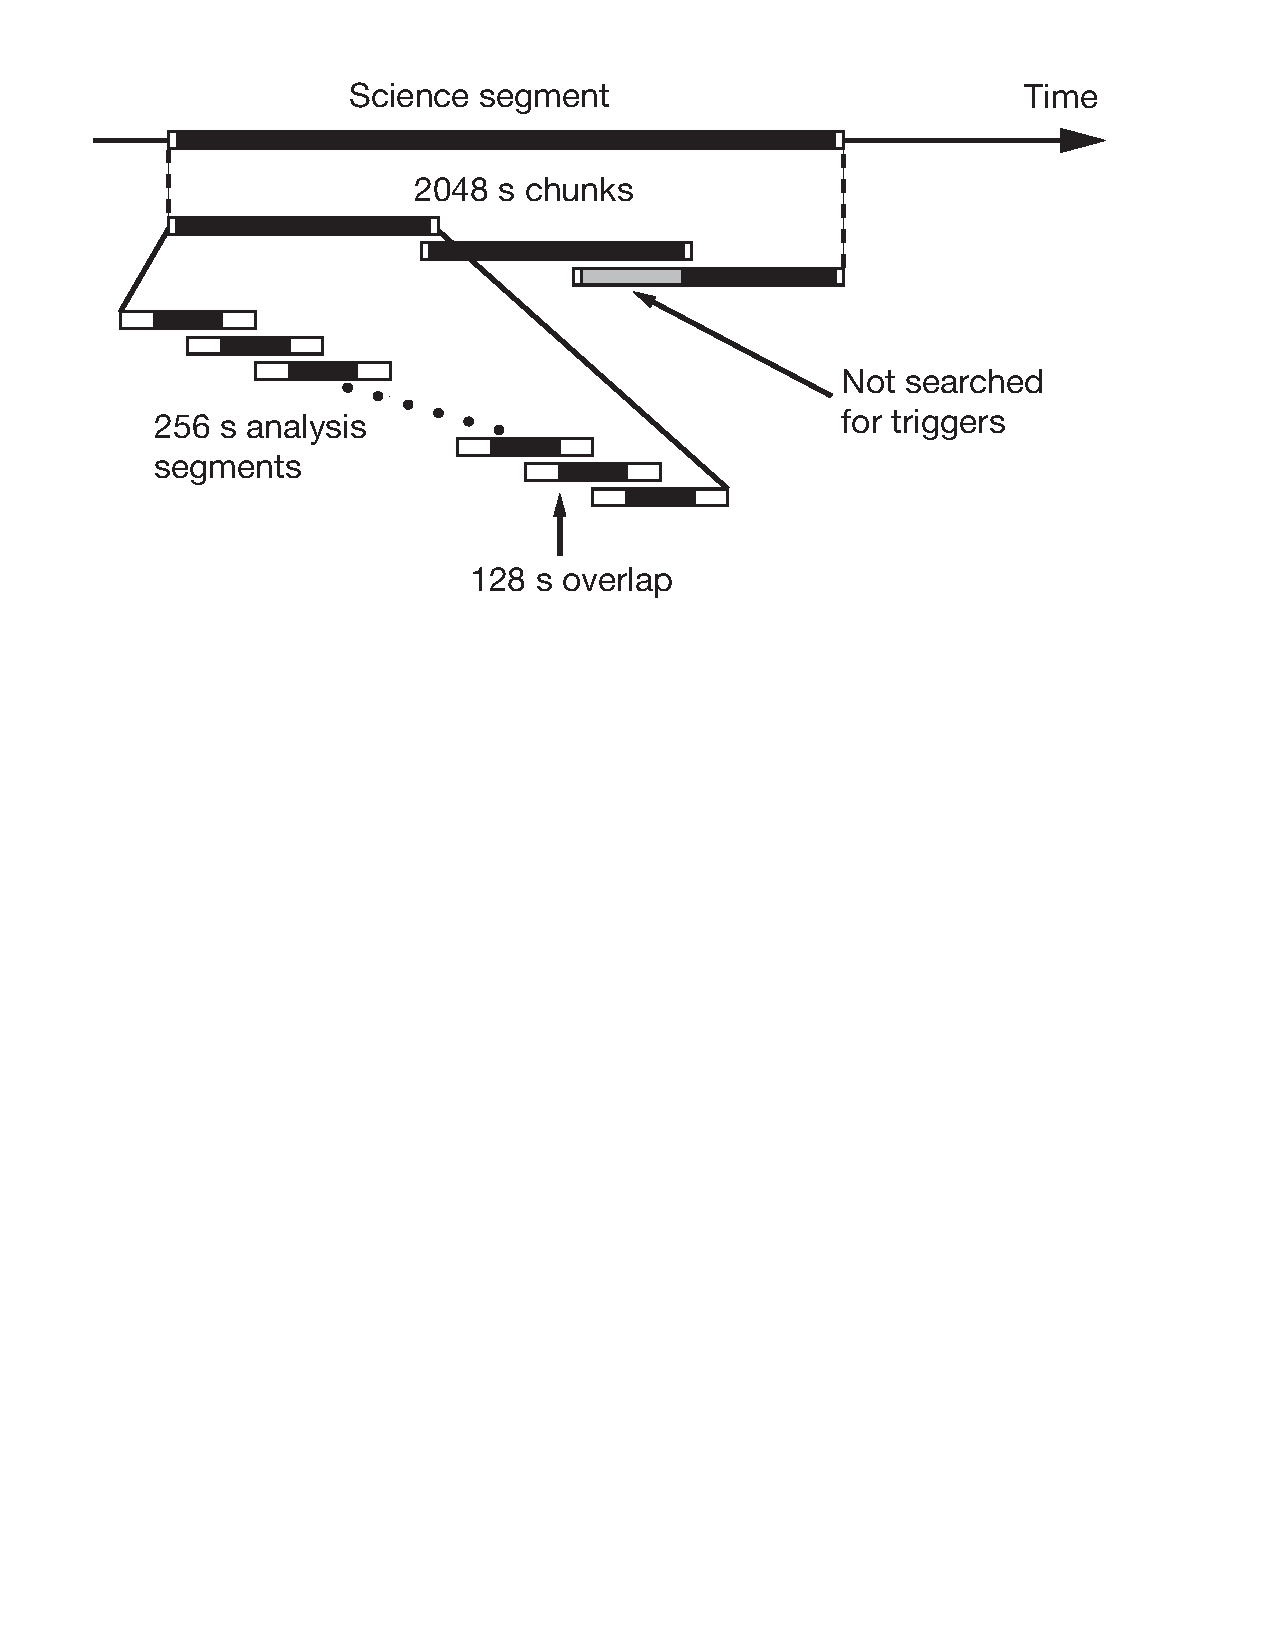
\includegraphics[width=\linewidth]{figures/pipeline/s2_segments}
\end{center}
\caption{%
The algorithm used to divide science segments into data analysis segments.
Science segments are divided into $2048$~s chunks overlapped by $128$~s.
(Science segments shorter than $2048$~s are ignored.) An additional chunk with
a larger overlap is added to cover any remaining data at the end of a science
segment.  Each chunk is divided into $15$ analysis segments of length $256$~s
for filtering. The first and last $64$~s of each analysis segment is ignored,
so the segments overlap by $128$~s.  Areas shaded black are filtered for
triggers by the search pipeline. The gray area in the last chunk of the
science segment is not searched for triggers as this time is covered by the
preceding chunk, however this data is used in the PSD estimate for the final
chunk.
}
\end{figure}

\section{Auxiliary and Environmental Vetoes}
\label{s:dq}

The other method was to look for signatures in environmental monitoring
channels and auxiliary interferometer channels which would indicate an
external disturbance or instrumental ``glitch'', allowing us to {\it veto} any
triggers recorded at that time.

Auxiliary interferometer channels (which monitor the light in the
interferometer at points other than the antisymmetric port---where a
gravitational wave would be most evident) were examined, with the aim being to
look for correlations between glitches found in the readouts of these channels
and inspiral event triggers found in the playground data.  By doing so, we are
capable of identifying instrumental artifacts that directly affect the light
that is measured in the gravitational wave channel, so these vetoes are
potentially very powerful.  However, we had to consider the possibility that a
gravitational wave itself could produce the observed glitches in the auxiliary
channel due to some physical or electronic coupling.  This possibility was
tested by means of {\em hardware} injections, in which a simulated inspiral
signal is injected into the interferometer by physically moving one of the end
mirrors of the interferometer. Hardware injections allow us to establish a
limit on the effect that a true signal would have on the auxiliary channels.
Only those channels that were unaffected by the hardware injections were
considered ``safe'' for use as potential veto channels. Hardware injections
are described in more detail in chapter \ref{ch:hardware}.

We used a computer program, {\it glitchMon} \cite{glitchMon}, to examine the
data and identify large amplitude transient signals in auxiliary channels.
Numerous channels, with various filters and threshold settings, were examined
with glitchMon. The program produces a list of times when the glitches
occurred. The glitch event list was compared with times generated by triggers
from the inspiral search; all of these preliminary studies were conducted on
the playground data. A time window around a glitch was defined, and any
inspiral event within this window was rejected. One can associate the veto
with inspiral event candidates and evaluate a veto efficiency (percentage of
inspiral events eliminated), use percentage (percentage of veto triggers which
veto at least one inspiral event), and dead-time (percentage of science-data
time eliminated by the veto). The results of the veto invesitgations for
binary neutron stars are described in section \ref{s:} and for binary black
hole MACHOs in section \ref{s:}.

During investigation of inspiral triggers in the playground data, it was
discovered that many of the L1 inspiral triggers appeared to be the result of
non-stationary noise with frequency content around $70$~Hz.  An important
auxiliary channel, \texttt{L1:LSC-POB\_I}, proportional to the residual length
of the power recycling cavity, was found to have highly variable noise at
$70$~Hz.  There are understandable physical reasons for this, namely the power
recycling servo loop (for which \texttt{L1:LSC-POB\_I} is the error signal)
has a known instability around $70$~Hz, which often results in the appearance
of glitches in the detector output channel at around $70$~Hz.  As a
consequence, it was decided that the low-frequency cutoff of the binary
neutron star inspiral search should be set to $100$~Hz to reduce sensitivity
to these glitches.  This subsequently reduced the number of inspiral triggers
(presumably created by this problem); an inspection of artificial signals
injected into the interferometer revealed a very small loss of efficiency for
binary neutron star inspiral and BBHMACHO signal detection resulting from the
increase in the low frequency cutoff.

\section{Data Analysis Pipeline}
\label{s:pipeline}

The detection of a gravitational-wave inspiral signal in the S2 data would
(at the least) require triggers in both L1 and one or more of the Hanford
instruments with consistent arrival times (separated by less than the light
travel time between the detectors) and waveform parameters.  Requiring
temporal coincidence between the two observatories greatly reduces the
background rate due to spurious triggers. Demanding that a trigger is
detected in both the Livingston and Hanford detectors allows us to further
reduce the rate of spurious triggers due to correlated noise sources in the
Hanford detectors. When detectors at both observatories are operating
simultaneously, we may obtain an estimate of the rate of background triggers
by time-shifting the Hanford triggers with respect to the L1 triggers and
looking for coincident events between the shifted and unshifted triggers, as
described in section~\ref{ss:background}. 

During the S2 run, the three LIGO detectors had substantially different
sensitivities, as can be seen from figure \ref{f:s2noisecurve}. The
sensitivity of the L1 detector was greater than those of the Hanford detectors
throughout the run. Since the orientations of the LIGO interferometers are
similar, we expect that signals of astrophysical origin detected in the
Hanford interferometers are detectable in the L1 interferometer.  We use this
and the requirement that a signal be detected in both the Livingston and at
least one of the Hanford interferometers to construct a {\em triggered search}
pipeline, summarized in Fig.~\ref{f:pipeline}. We search for inspiral triggers
in the most sensitive interferometer (L1), and only when a trigger is found in
this interferometer do we search for a coincident trigger in the less
sensitive interferometers. This approach reduces the computational power
necessary to perform the search.

\begin{figure}[tbh]
  \vspace{5pt}
  \begin{flushright}
    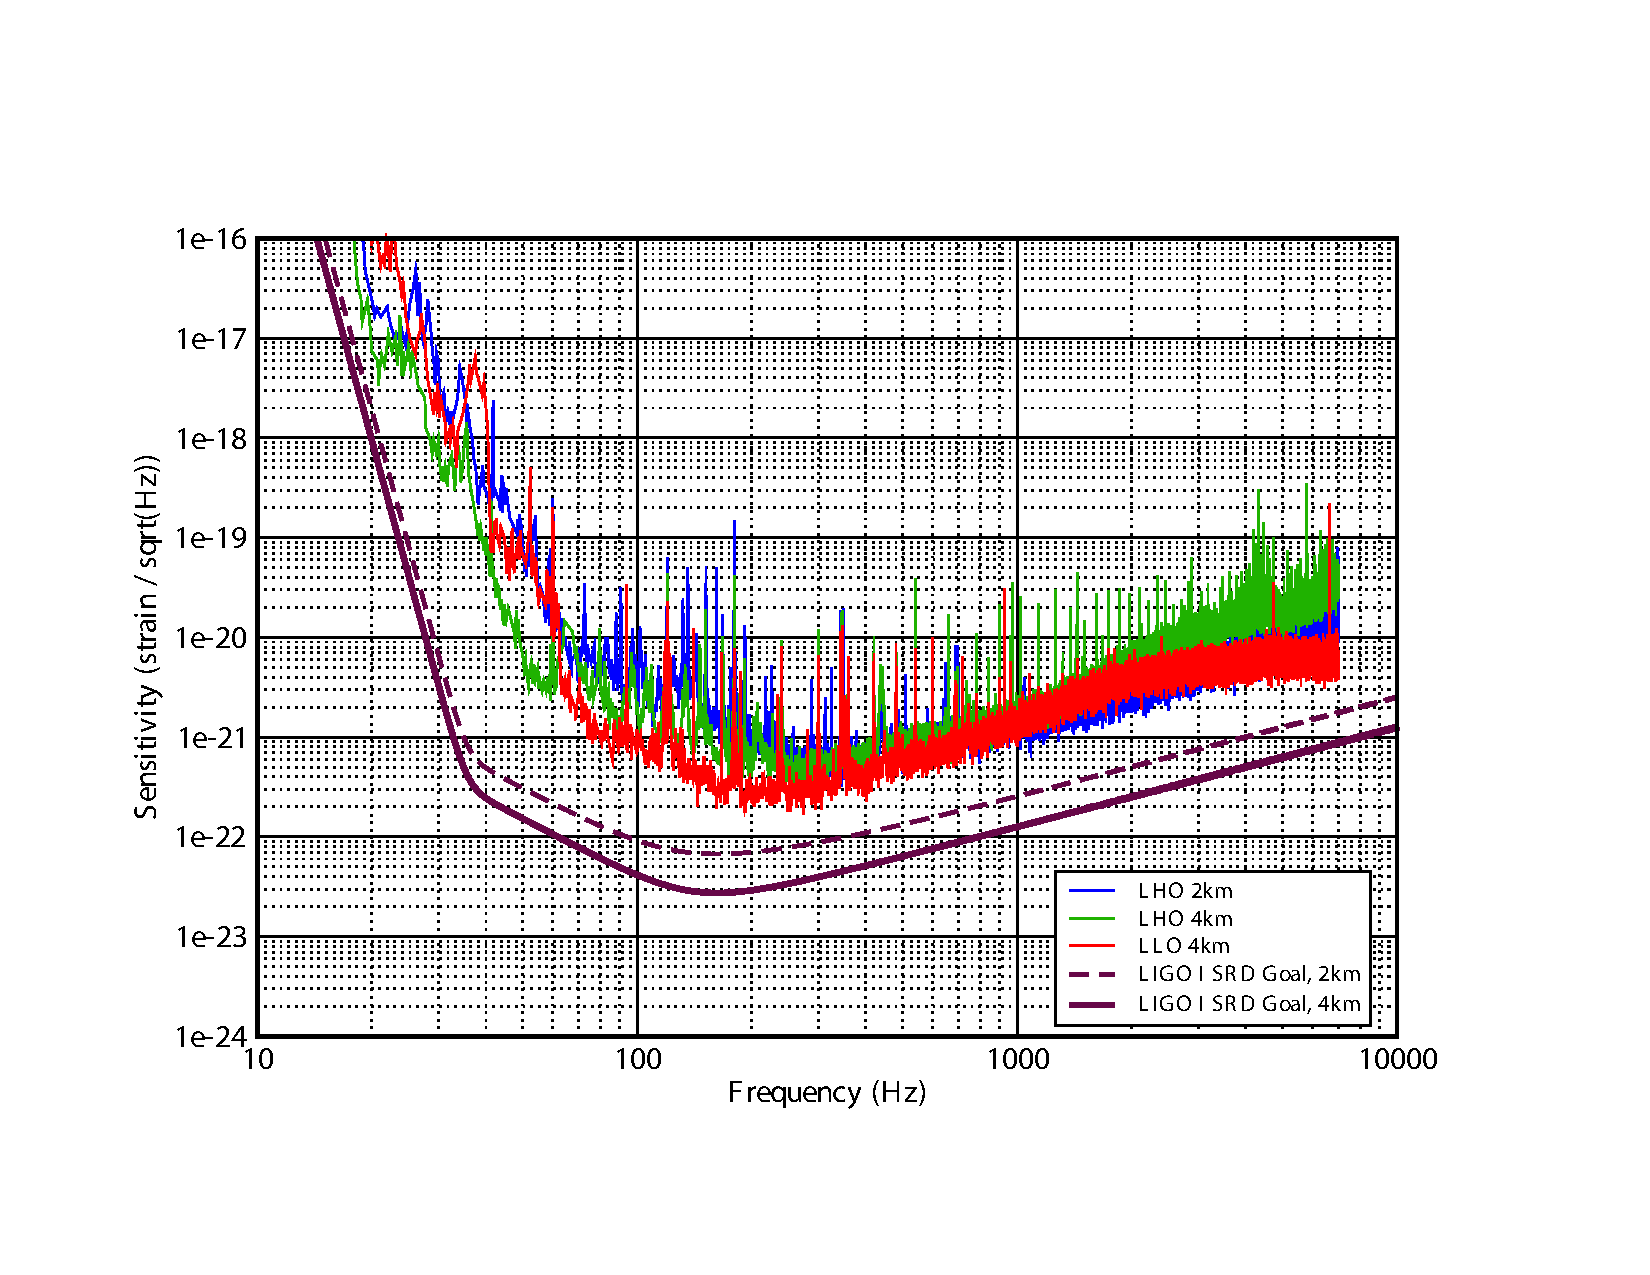
\includegraphics[width=\textwidth]{figures/pipeline/G030379-00}    
  \end{flushright}
  \caption{%
  Typical sensitivities of the three LIGO interferometers during the second
  LIGO science run\cite{s2noisecurve} shown as strain amplitude spectral
  density, $\tilde{h}/\sqrt{\mathrm{Hz}}$. The smooth solid curve shows the
  design sensitivity (SRD Goal) of the $4$~km interferometers and the smooth
  dashed curve shows the design sensitivity of the $2$~km interferometer.
  }
\label{f:s2noisecurve}
\end{figure}

\begin{figure}
\begin{center}
\hspace*{-0.2in}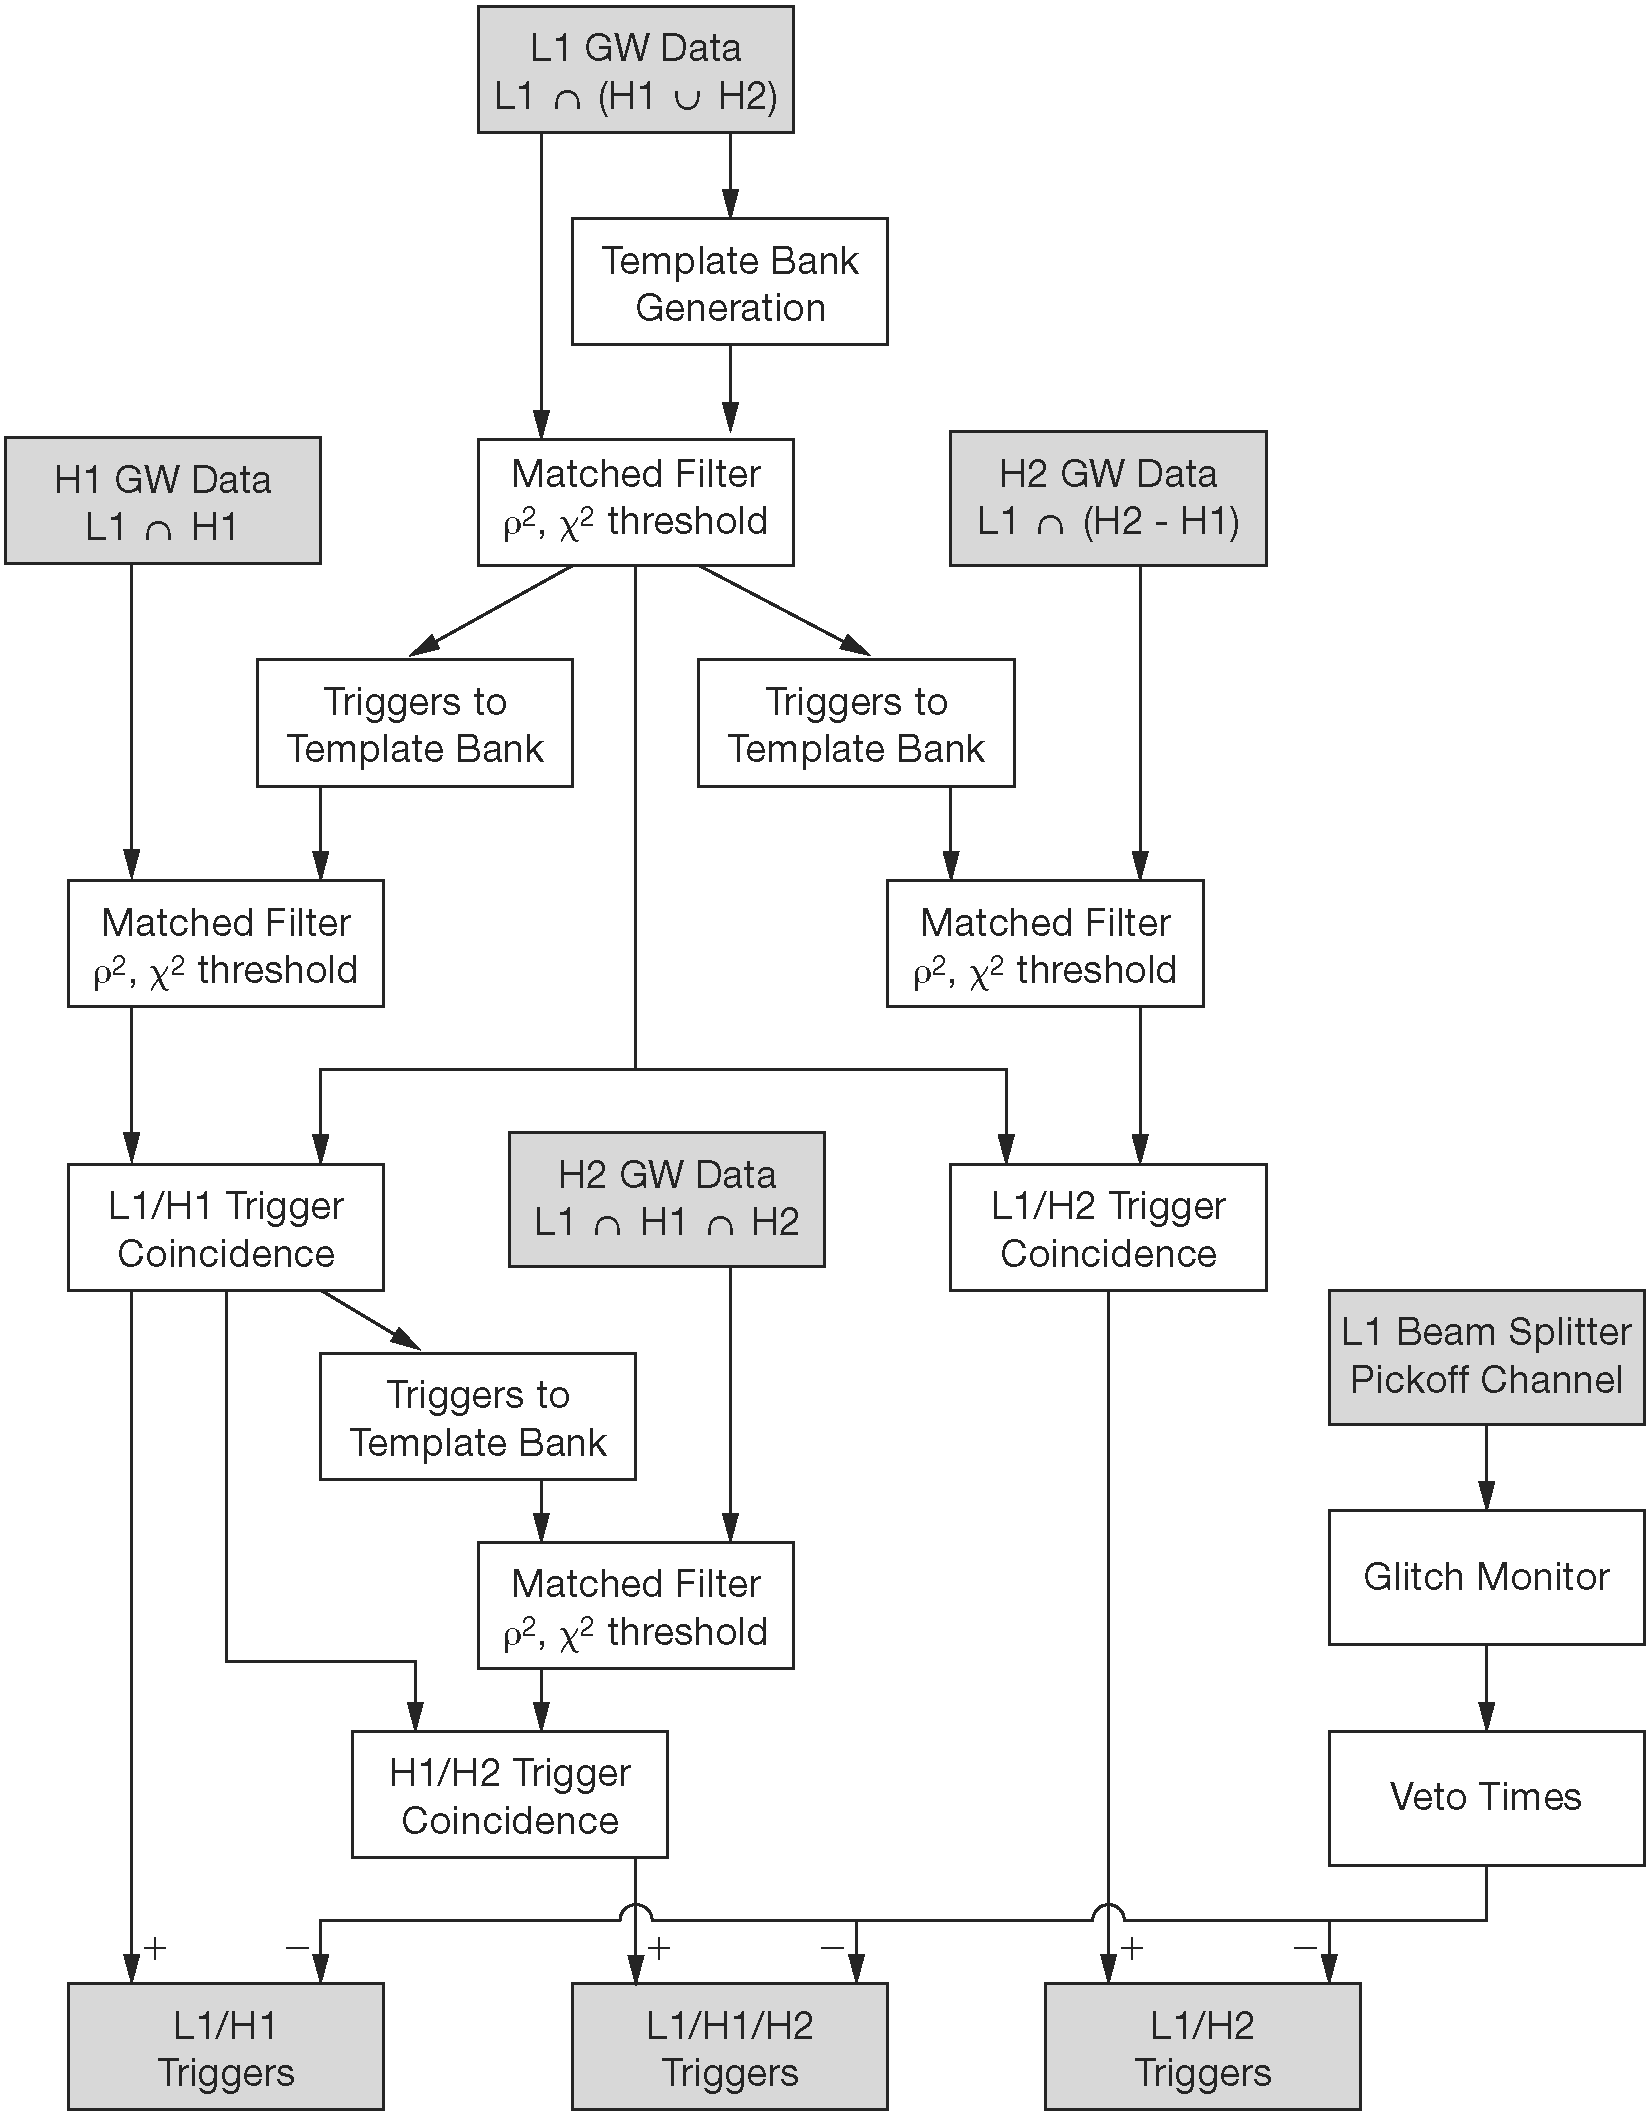
\includegraphics[width=\linewidth]{figures/pipeline/s2_pipeline}
\end{center}
\caption{\label{f:pipeline}%
The inspiral analysis pipeline used to determine the reported upper
limit. $\mathrm{L1} \cap (\mathrm{H1} \cup \mathrm{H2})$ indicates times when
the L1 interferometer was operating in coincidence with one or both of the
Hanford interferometers. $\mathrm{L1} \cap \mathrm{H1}$ indicates times when
the L1 interferometer was operating in coincidence with the H1 interferometer.
$\mathrm{L1} \cap (\mathrm{H2} - \mathrm{H1})$ indicates times when the L1
interferometer was operating in coincidence with only the H2 interferometer.
The outputs of the search pipeline are triggers that belong to one of the
two double coincident data sets or to the triple coincident data set.}
\end{figure}

The power spectral density (PSD) of the noise in the Livingston detector is
estimated independently for each L1 chunk that is coincident with operation of
a Hanford detector (denoted $\mathrm{L1} \cap (\mathrm{H1} \cup
\mathrm{H2}$)).  The PSD is used to lay out a template bank for filtering that
chunk, according to the parameters for mass ranges and minimal
match\cite{Owen:1998dk}. The data from the L1 interferometer for the chunk is
then filtered, using that bank, with a signal-to-noise threshold
$\rho_{\mathrm{L}}^\ast$ and $\chi^2$ veto threshold
$\chi^2_{\ast\mathrm{L}}$ to produce a list of triggers as described in
section~\ref{s:triggers}.  For each chunk in the Hanford interferometers, a
{triggered bank} is created by adding a template if it produced at least one
trigger in L1 during the time of the Hanford chunk.  This is used to filter
the data from the Hanford interferometers with signal-to-noise and $\chi^2$
thresholds specific to the interferometer, giving a total of six thresholds
that may be tuned.  For times when only the H2 interferometer is operating in
coincidence with L1 (denoted $\mathrm{L1} \cap (\mathrm{H2} - \mathrm{H1}$)
the triggered bank is used to filter the H2 chunks that overlap with L1 data;
these triggers are used to test for L1/H2 double coincidence.  All H1 data
that overlaps with L1 data (denoted $\mathrm{L1} \cap \mathrm{H1}$) is
filtered using the triggered bank for that chunk. For H1 triggers produced
during times when all three interferometers are operating, a second triggered
bank is produced for each H2 chunk by adding a template if it produced at
least one trigger found in coincidence in L1 and H1 during the time of the H2
chunk and the H2 chunk is filtered with this bank.  These triggers are used to
search for triple coincident triggers in H2.  The remaining triggers from H1
when H2 is not available are used to search for L1/H1 double coincident
triggers.


\section{Trigger Coincidence}
\label{s:coincidence}

For a trigger to be considered coincident in two interferometers, we demand
that it is observed in both interferometers within a temporal coincidence
window, $\delta t$, that allows for the error in measurement of the time of the trigger. Monte Carlo analysis with simulated signals suggests that we
cannot measure the time of the trigger to an accuracy of less than $1$~ms, so
we demand $\delta t = 1$~ms if the interferometers are located at the same
observatory. If the detectors are not co-located, we allow for the $10$~ms
light travel time between the LIGO observatories by demanding $\delta t =
11$~ms. We also demand that the waveform of the triggers are consistent by
requiring that the two mass parameters, $m_1$ and $m_2$, of the binary are
identical to within an error of $\delta m$.

\begin{figure}
  \vspace{5pt}
  \begin{flushright}
    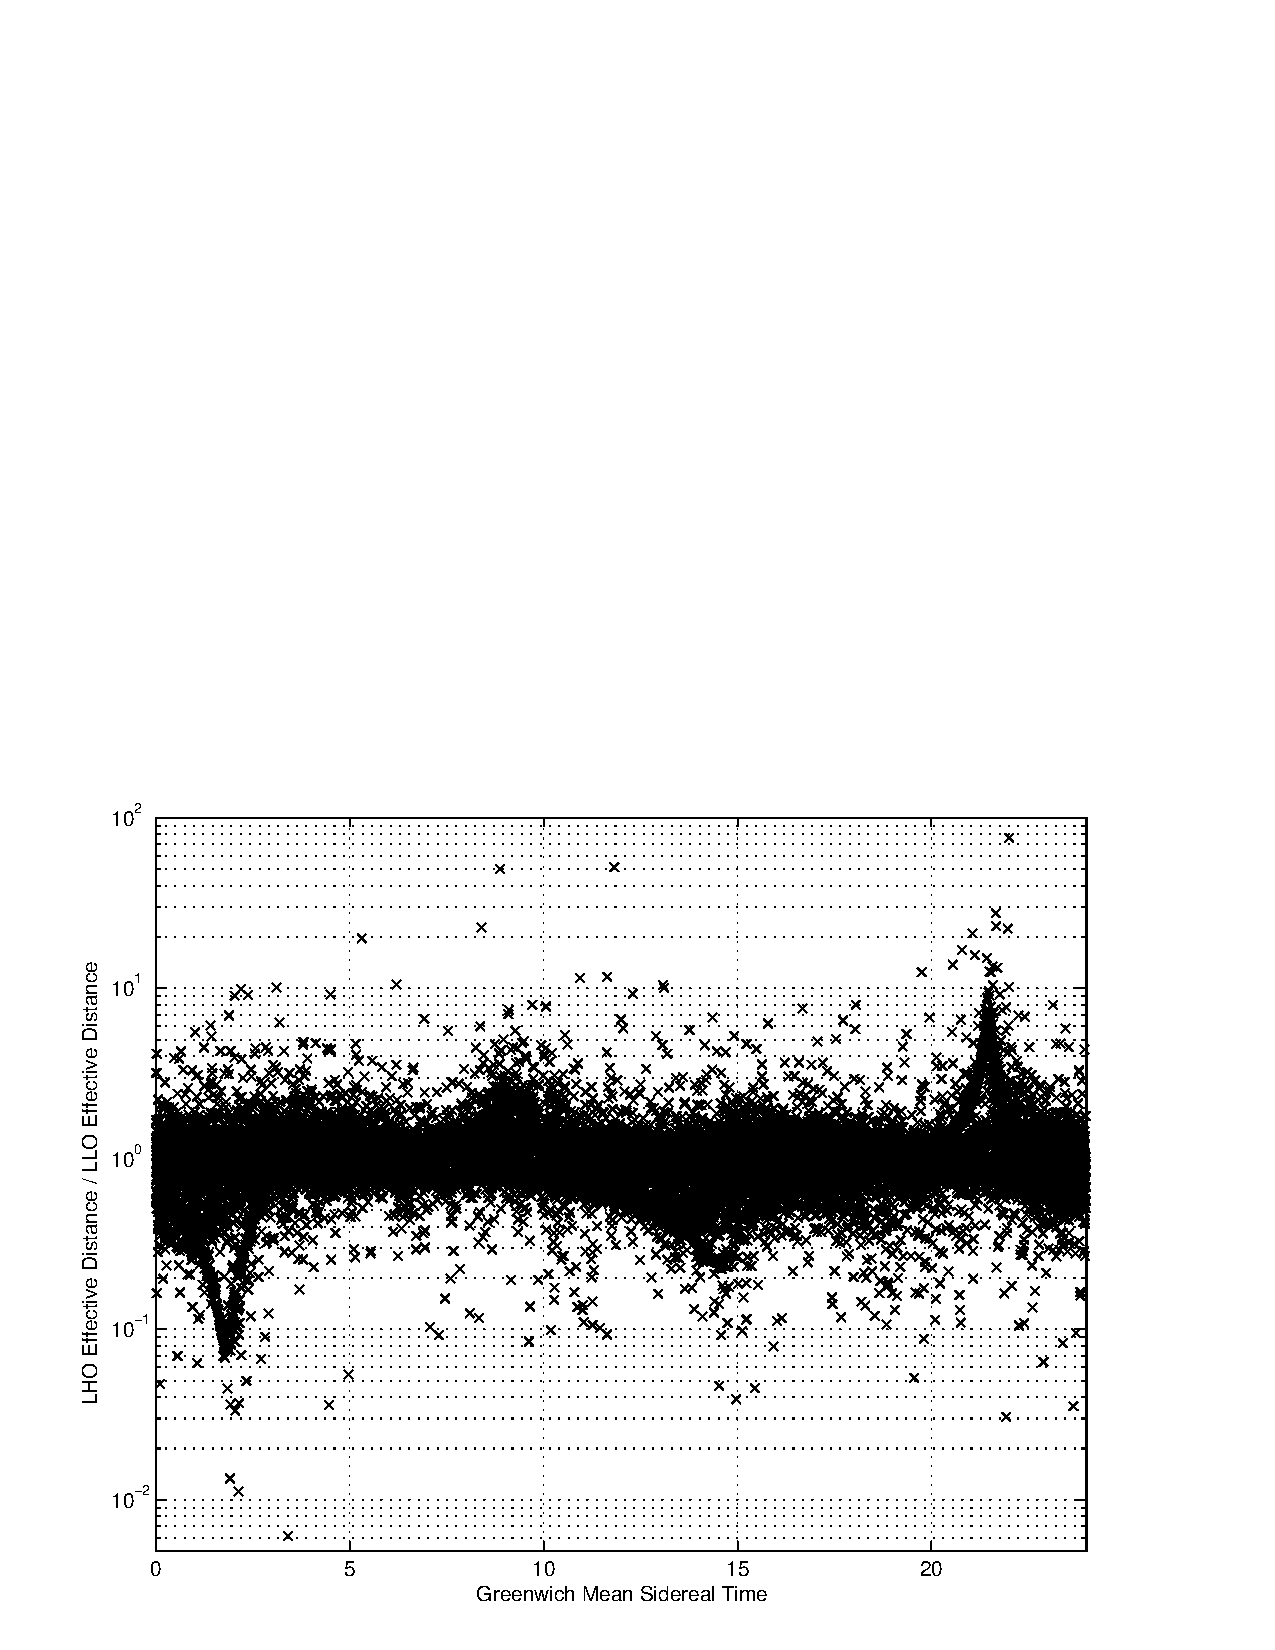
\includegraphics[width=\textwidth]{figures/pipeline/gmst_dist_ratio}    
  \end{flushright}
  \caption{%
  The ratio of the known effective distance of an injected signal in the
  Hanford Observatory (LHO) to the known effective distance of an injected
  signal in the Livingston Observatory (LLO) as a function of Greenwich Mean
  Sidereal Time. The slight misalignment of the interferometers at the two
  different observatories due to the curvature of the earth causes the antenna
  pattern of the detectors to differ. As a result the distance at which a
  binary system appears is different in each detector, even in the absence of
  noise.  The ratio of effective distances can be significant, so this
  precludes the use of an amplitude cut when testing for inspiral trigger
  coincidence between different observatories.
  }
\label{f:gmst_dist_ratio}
\end{figure}
We now consider an amplitude cut on the signals. The Livingston and Hanford
detectors are not co-aligned. There is a slight misalignment of the detectors
due to the curvature of the earth and so the antenna patterns of the detectors
differ. This causes the measured amplitude of a gravitational wave to differ
between the sites. In the extreme case, it is possible for a binary to be
completely undetectable by the L1 detector, but still detectable by the H1 and
H2 detectors. For a given inspiral trigger, we measure the \emph{effective
distance} of the binary system. This is the distance at which an optimally
oriented binary would produce the observed signal-to-noise ratio.
Figure~\ref{f:gmst_dist_ratio} shows the ratio of effective distances between
the two LIGO observatories for the population of binary neutron stars
considered in the S2 analysis. The significant variation of the effective
distance precludes using a naive test for amplitude coincidence. It is
possible to obtain information about sky position from time delay between
sites to construct a more complicated amplitude cut, but this has not be used
in the S2 analysis.

In the case of triggers from the H1 and H2 interferometers that are coincident
in time and mass, we apply an amplitude cut that tests that the effective
distance of the triggers is coincident given the relative sensitivity of the
detectors, while allowing for error in this measurement which is determined by
Monte Carlo simulations.  When testing for triple coincident triggers we 
accept triggers that are coincident in the L1 and H1 detectors that are
\emph{not} present in the H2 detector \emph{if} the effective distance of the
trigger is further than the maximum distance of H2 at signal-to-noise ratio
$6$ at the time of the candidate trigger. Figure \ref{f:coinc_test} sumarizes
the time, mass and distance coincidence test.  The final step of the pipeline
is to apply and auxiliary interferometer vetoes described in
section~\ref{s:vetoes}. 

The list of surviving candidate triggers is followed up by examining the raw
gravitational wave data, axillary interferometer channels and physical
environment monitoring channels to determine if the triggers are truly of
astrophysical origin.

\begin{figure}
\begin{center}
\hspace*{-0.2in}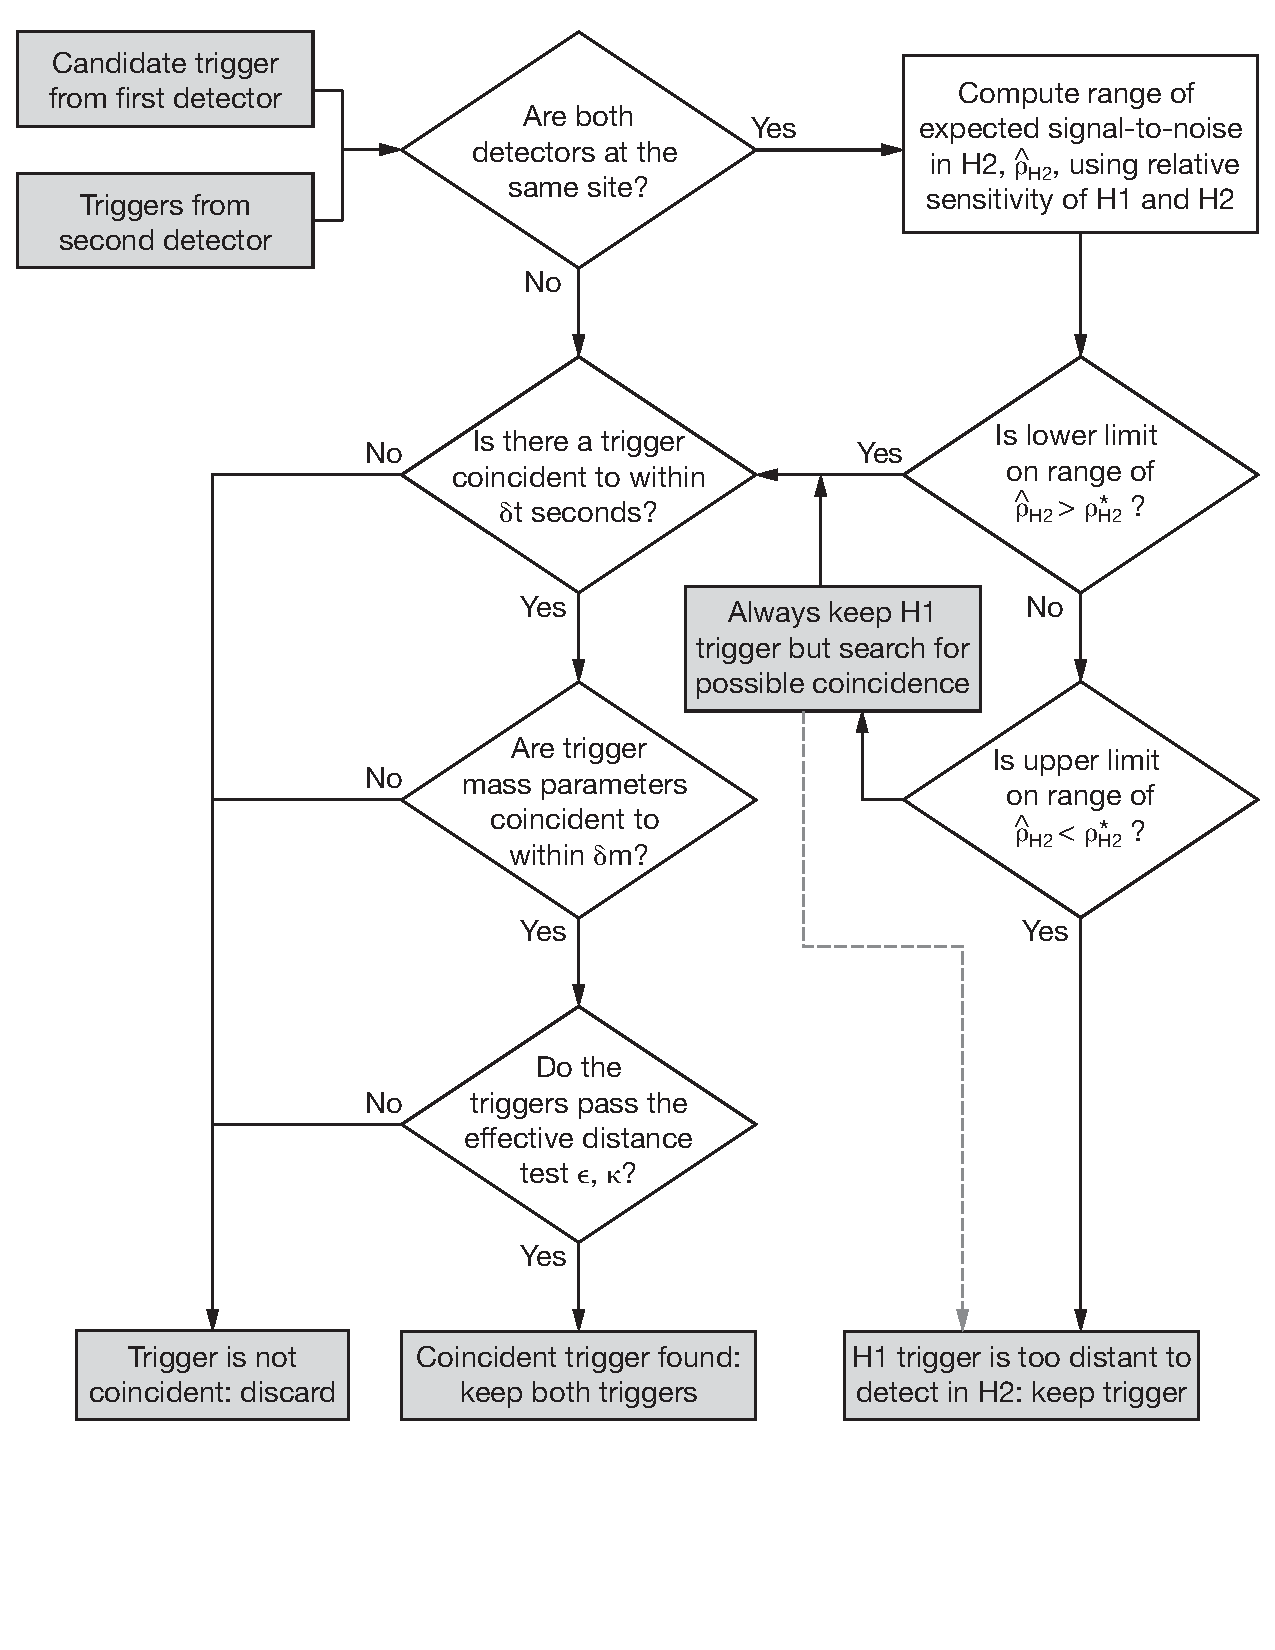
\includegraphics[width=\linewidth]{figures/pipeline/s2_coinc_test}
\end{center}
\caption{\label{f:coinc_test}%
The test to decide if a trigger in the first detector has a coincident 
trigger in the second detector. If detectors are at different sites, time and
mass coincidence are demanded. The effective distance cut is disabled by 
setting $\kappa = 1000$. If the detectors are at the same site, we ask if the
maximum distance to which H2 can see at the signal-to-noise threshold
$\rho_\mathrm{H2}^\ast$ is greater than the distance of the H1 trigger,
allowing for errors in the measurement of the trigger distance. If this is the
case, we demand time, mass and effective distance coincidence.  If distance to
which H2 can see overlaps the error in measured distance of the H1 trigger, we
search for a trigger in H2, but always keep the H1 trigger even if no
coincident trigger is found. If the minimum of the error in measured distance
of the H1 trigger is greater than the maximum distance to which H2 can detect
a trigger we keep the H1 trigger without searching for coincidence.}
\end{figure}

\section{Background Estimation}
\label{s:background}

Since we restrict the S2 analysis to coincident data and require that at least
two of the interferometers must be located at different observatories, we may
measure a background rate for our analysis. After generating triggers for each
interferometer, we slide the triggers from one observatory relative to the
other observatory and look for coincidences between the shifted and unshifted
triggers. The minimum slide length is chosen to be greater than the length of
the longest filter ($20$~sec) so any coincident triggers detected must be due to background and
not astrophysical events. By examining the distribution of background events
in the $(\rho_\mathrm{H},\rho_\mathrm{L})$ plane we can attempt to determine
contours of constant false alarm rate in order to construct a combined
effective signal-to-noise ratio for a coincident trigger\cite{abbott2004a}.

\section{Detection Efficiency}
\label{s:eff}

In absence of detection, we will construct an upper limit on event rate.  To
do this, need to measure the detection efficiency of the analysis pipeline to
our population. A Monte Carlo method is used to measure this efficiency. We
simulate a population of binary neutron stars and \emph{inject} signals from
that population into the data from all three LIGO interferometers. The
injection is performed in software by generating an inspiral waveform and
adding it to interferometer data immediately after the raw data is read from
disk. We inject the actual waveform that would be detected in a given
interferometer accounting for both the masses, orientation, polarization, sky
position and distance of the binary, the antenna pattern and calibration of
the interferometer into which this signal is injected.  The effectiveness of
software injections for measuring the response of the instrument to an
inspiral signal is validated against \emph{hardware injections}\cite{hw} where
an inspiral signal is added to the interferometer control servo during
operation to produce the same output signal as a real gravitational wave.  The
data with injections is run through the full analysis pipeline to produce a
list of inspiral triggers. The detection efficiency of the pipeline,
$\epsilon$, is the ratio of the number of detected signals to the number of
injected signals.
